% 插值搜索
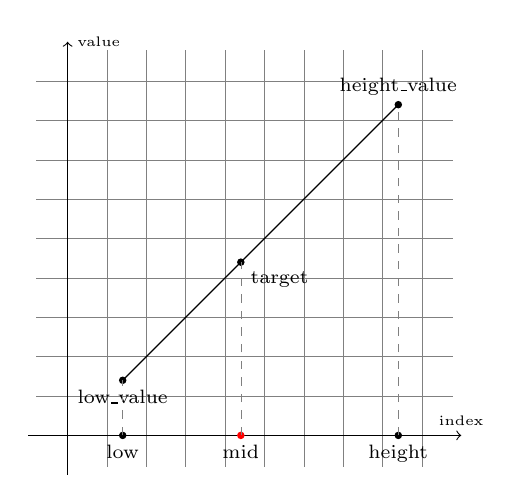
\begin{tikzpicture}
  \tikzstyle{every node}=[font=\scriptsize]

  \draw[step=.5cm,gray,very thin] (-0.4,-0.4) grid (4.9,4.9);
  \draw [->] (-0.5,0) -- (5,0);
  \node [above] at (5,0) {\tiny index};
  \draw [->] (0,-0.5) -- (0,5);
  \node [right] at (0,5) {\tiny value};
  \draw (0.7,0.7) -- (4.2,4.2);

  \draw[fill] (0.7,0.7) circle [radius=0.04];
  \node [below] at (0.7,0.7) {low\_value};
  \draw[fill] (0.7,0) circle [radius=0.04];
  \node [below] at (0.7,0) {low};

  \draw[fill] (2.2,2.2) circle [radius=0.04];
  \node [below right] at (2.2,2.2) {target};
  \draw[fill,red] (2.2,0) circle [radius=0.04];
  \node [below] at (2.2,0) {mid};

  \draw[fill] (4.2,4.2) circle [radius=0.04];
  \node [above] at (4.2,4.2) {height\_value};
  \draw[fill] (4.2,0) circle [radius=0.04];
  \node [below] at (4.2,0) {height};

  \draw[dashed,gray,very thin] (0.7,0) -- (0.7,0.7);
  \draw[dashed,gray,very thin] (2.2,0) -- (2.2,2.2);
  \draw[dashed,gray,very thin] (4.2,0) -- (4.2,4.2);
\end{tikzpicture}
